\documentclass[1p]{elsarticle_modified}
%\bibliographystyle{elsarticle-num}

%\usepackage[colorlinks]{hyperref}
%\usepackage{abbrmath_seonhwa} %\Abb, \Ascr, \Acal ,\Abf, \Afrak
\usepackage{amsfonts}
\usepackage{amssymb}
\usepackage{amsmath}
\usepackage{amsthm}
\usepackage{scalefnt}
\usepackage{amsbsy}
\usepackage{kotex}
\usepackage{caption}
\usepackage{subfig}
\usepackage{color}
\usepackage{graphicx}
\usepackage{xcolor} %% white, black, red, green, blue, cyan, magenta, yellow
\usepackage{float}
\usepackage{setspace}
\usepackage{hyperref}

\usepackage{tikz}
\usetikzlibrary{arrows}

\usepackage{multirow}
\usepackage{array} % fixed length table
\usepackage{hhline}

%%%%%%%%%%%%%%%%%%%%%
\makeatletter
\renewcommand*\env@matrix[1][\arraystretch]{%
	\edef\arraystretch{#1}%
	\hskip -\arraycolsep
	\let\@ifnextchar\new@ifnextchar
	\array{*\c@MaxMatrixCols c}}
\makeatother %https://tex.stackexchange.com/questions/14071/how-can-i-increase-the-line-spacing-in-a-matrix
%%%%%%%%%%%%%%%

\usepackage[normalem]{ulem}

\newcommand{\msout}[1]{\ifmmode\text{\sout{\ensuremath{#1}}}\else\sout{#1}\fi}
%SOURCE: \msout is \stkout macro in https://tex.stackexchange.com/questions/20609/strikeout-in-math-mode

\newcommand{\cancel}[1]{
	\ifmmode
	{\color{red}\msout{#1}}
	\else
	{\color{red}\sout{#1}}
	\fi
}

\newcommand{\add}[1]{
	{\color{blue}\uwave{#1}}
}

\newcommand{\replace}[2]{
	\ifmmode
	{\color{red}\msout{#1}}{\color{blue}\uwave{#2}}
	\else
	{\color{red}\sout{#1}}{\color{blue}\uwave{#2}}
	\fi
}

\newcommand{\Sol}{\mathcal{S}} %segment
\newcommand{\D}{D} %diagram
\newcommand{\A}{\mathcal{A}} %arc


%%%%%%%%%%%%%%%%%%%%%%%%%%%%%5 test

\def\sl{\operatorname{\textup{SL}}(2,\Cbb)}
\def\psl{\operatorname{\textup{PSL}}(2,\Cbb)}
\def\quan{\mkern 1mu \triangleright \mkern 1mu}

\theoremstyle{definition}
\newtheorem{thm}{Theorem}[section]
\newtheorem{prop}[thm]{Proposition}
\newtheorem{lem}[thm]{Lemma}
\newtheorem{ques}[thm]{Question}
\newtheorem{cor}[thm]{Corollary}
\newtheorem{defn}[thm]{Definition}
\newtheorem{exam}[thm]{Example}
\newtheorem{rmk}[thm]{Remark}
\newtheorem{alg}[thm]{Algorithm}

\newcommand{\I}{\sqrt{-1}}
\begin{document}

%\begin{frontmatter}
%
%\title{Boundary parabolic representations of knots up to 8 crossings}
%
%%% Group authors per affiliation:
%\author{Yunhi Cho} 
%\address{Department of Mathematics, University of Seoul, Seoul, Korea}
%\ead{yhcho@uos.ac.kr}
%
%
%\author{Seonhwa Kim} %\fnref{s_kim}}
%\address{Center for Geometry and Physics, Institute for Basic Science, Pohang, 37673, Korea}
%\ead{ryeona17@ibs.re.kr}
%
%\author{Hyuk Kim}
%\address{Department of Mathematical Sciences, Seoul National University, Seoul 08826, Korea}
%\ead{hyukkim@snu.ac.kr}
%
%\author{Seokbeom Yoon}
%\address{Department of Mathematical Sciences, Seoul National University, Seoul, 08826,  Korea}
%\ead{sbyoon15@snu.ac.kr}
%
%\begin{abstract}
%We find all boundary parabolic representation of knots up to 8 crossings.
%
%\end{abstract}
%\begin{keyword}
%    \MSC[2010] 57M25 
%\end{keyword}
%
%\end{frontmatter}

%\linenumbers
%\tableofcontents
%
\newcommand\colored[1]{\textcolor{white}{\rule[-0.35ex]{0.8em}{1.4ex}}\kern-0.8em\color{red} #1}%
%\newcommand\colored[1]{\textcolor{white}{ #1}\kern-2.17ex	\textcolor{white}{ #1}\kern-1.81ex	\textcolor{white}{ #1}\kern-2.15ex\color{red}#1	}

{\Large $\underline{12n_{0404}~(K12n_{0404})}$}

\setlength{\tabcolsep}{10pt}
\renewcommand{\arraystretch}{1.6}
\vspace{1cm}\begin{tabular}{m{100pt}>{\centering\arraybackslash}m{274pt}}
\multirow{5}{120pt}{
	\centering
	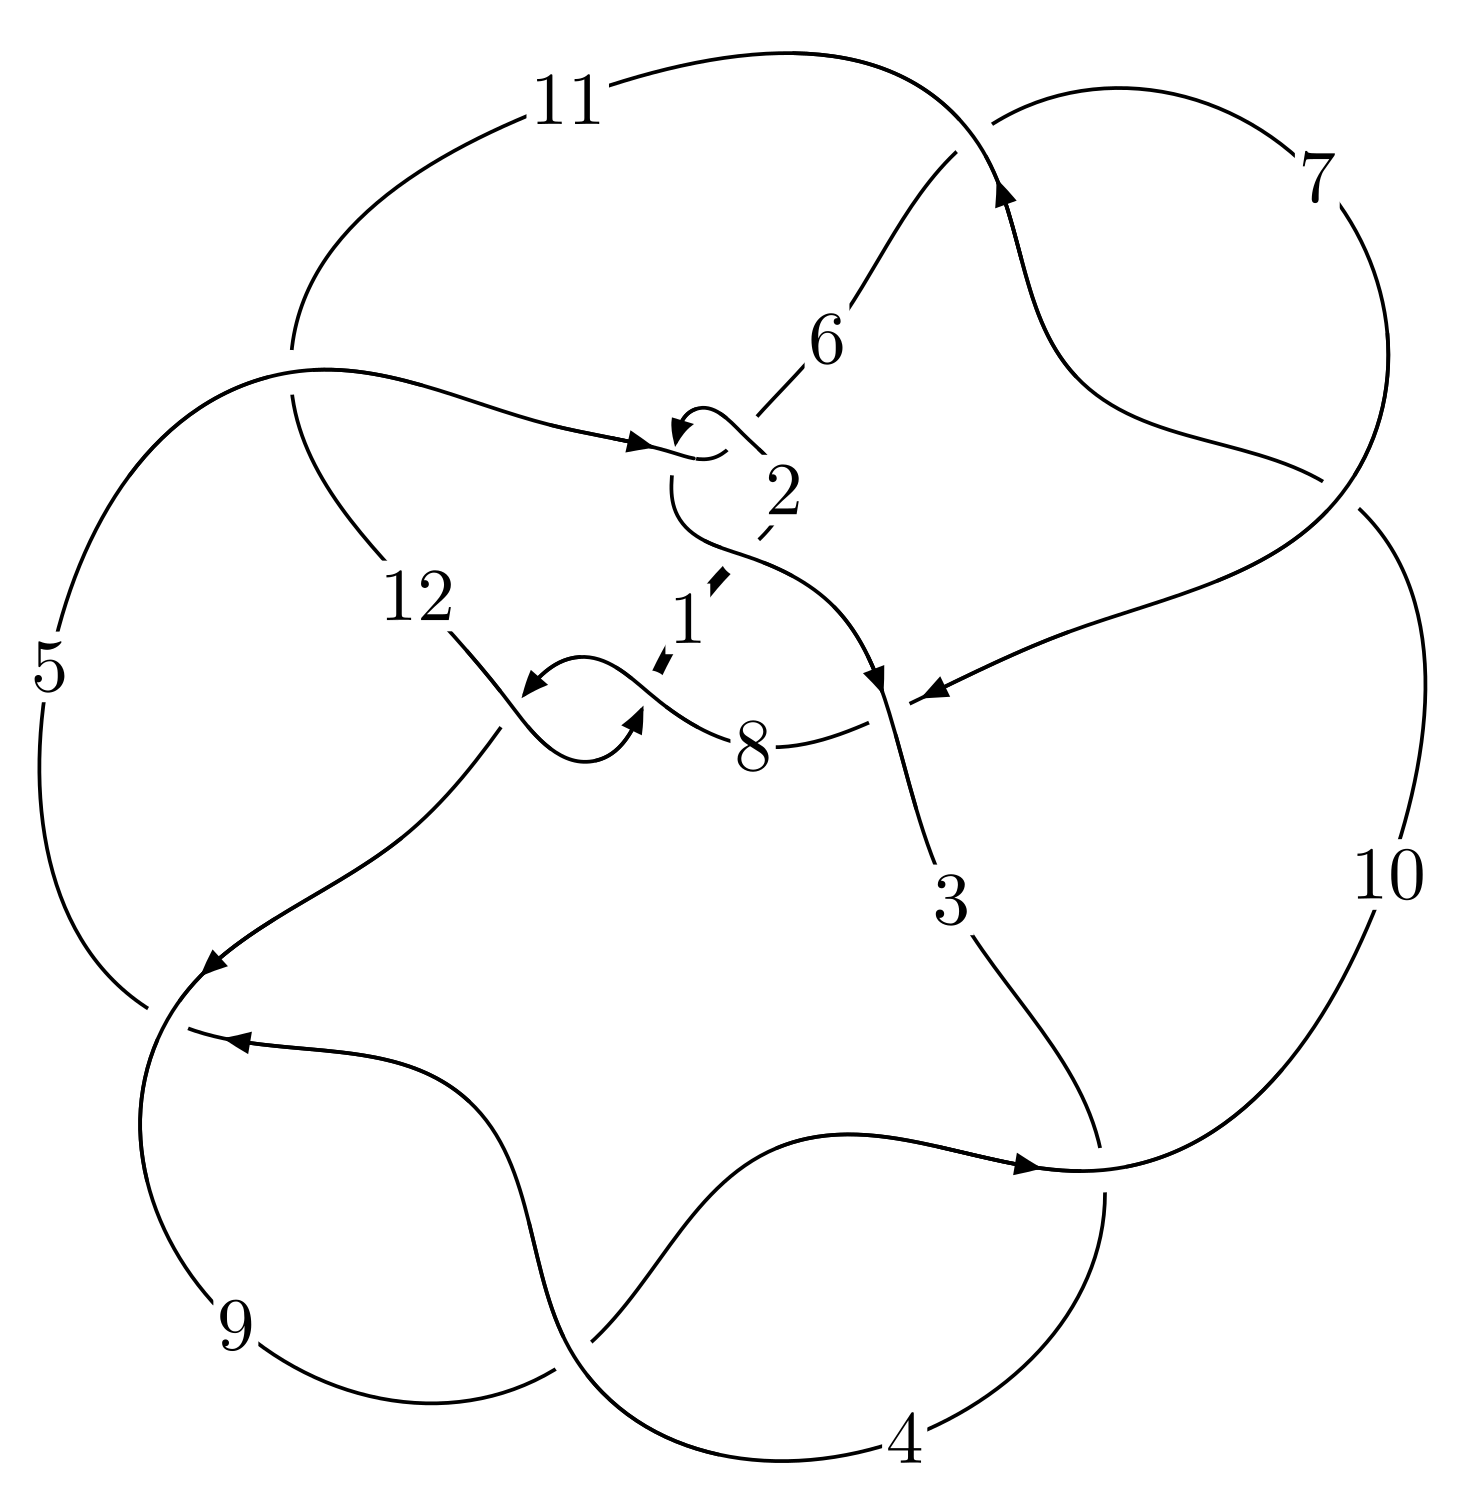
\includegraphics[width=112pt]{../../../GIT/diagram.site/Diagrams/png/2493_12n_0404.png}\\
\ \ \ A knot diagram\footnotemark}&
\allowdisplaybreaks
\textbf{Linearized knot diagam} \\
\cline{2-2}
 &
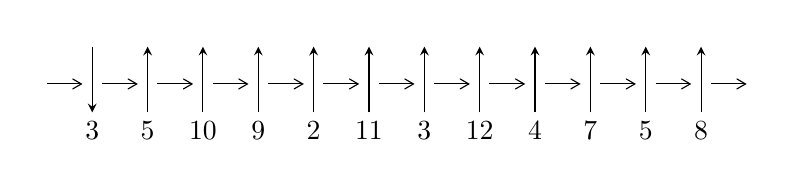
\begin{tikzpicture}[x=20pt, y=17pt]
	% nodes
	\node (C0) at (0, 0) {};
	\node (C1) at (1, 0) {};
	\node (C1U) at (1, +1) {};
	\node (C1D) at (1, -1) {3};

	\node (C2) at (2, 0) {};
	\node (C2U) at (2, +1) {};
	\node (C2D) at (2, -1) {5};

	\node (C3) at (3, 0) {};
	\node (C3U) at (3, +1) {};
	\node (C3D) at (3, -1) {10};

	\node (C4) at (4, 0) {};
	\node (C4U) at (4, +1) {};
	\node (C4D) at (4, -1) {9};

	\node (C5) at (5, 0) {};
	\node (C5U) at (5, +1) {};
	\node (C5D) at (5, -1) {2};

	\node (C6) at (6, 0) {};
	\node (C6U) at (6, +1) {};
	\node (C6D) at (6, -1) {11};

	\node (C7) at (7, 0) {};
	\node (C7U) at (7, +1) {};
	\node (C7D) at (7, -1) {3};

	\node (C8) at (8, 0) {};
	\node (C8U) at (8, +1) {};
	\node (C8D) at (8, -1) {12};

	\node (C9) at (9, 0) {};
	\node (C9U) at (9, +1) {};
	\node (C9D) at (9, -1) {4};

	\node (C10) at (10, 0) {};
	\node (C10U) at (10, +1) {};
	\node (C10D) at (10, -1) {7};

	\node (C11) at (11, 0) {};
	\node (C11U) at (11, +1) {};
	\node (C11D) at (11, -1) {5};

	\node (C12) at (12, 0) {};
	\node (C12U) at (12, +1) {};
	\node (C12D) at (12, -1) {8};
	\node (C13) at (13, 0) {};

	% arrows
	\draw[->,>={angle 60}]
	(C0) edge (C1) (C1) edge (C2) (C2) edge (C3) (C3) edge (C4) (C4) edge (C5) (C5) edge (C6) (C6) edge (C7) (C7) edge (C8) (C8) edge (C9) (C9) edge (C10) (C10) edge (C11) (C11) edge (C12) (C12) edge (C13) ;	\draw[->,>=stealth]
	(C1U) edge (C1D) (C2D) edge (C2U) (C3D) edge (C3U) (C4D) edge (C4U) (C5D) edge (C5U) (C6D) edge (C6U) (C7D) edge (C7U) (C8D) edge (C8U) (C9D) edge (C9U) (C10D) edge (C10U) (C11D) edge (C11U) (C12D) edge (C12U) ;
	\end{tikzpicture} \\
\hhline{~~} \\& 
\textbf{Solving Sequence} \\ \cline{2-2} 
 &
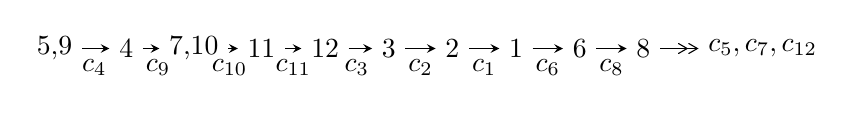
\begin{tikzpicture}[x=23pt, y=7pt]
	% node
	\node (A0) at (-1/8, 0) {5,9};
	\node (A1) at (1, 0) {4};
	\node (A2) at (33/16, 0) {7,10};
	\node (A3) at (25/8, 0) {11};
	\node (A4) at (33/8, 0) {12};
	\node (A5) at (41/8, 0) {3};
	\node (A6) at (49/8, 0) {2};
	\node (A7) at (57/8, 0) {1};
	\node (A8) at (65/8, 0) {6};
	\node (A9) at (73/8, 0) {8};
	\node (C1) at (1/2, -1) {$c_{4}$};
	\node (C2) at (3/2, -1) {$c_{9}$};
	\node (C3) at (21/8, -1) {$c_{10}$};
	\node (C4) at (29/8, -1) {$c_{11}$};
	\node (C5) at (37/8, -1) {$c_{3}$};
	\node (C6) at (45/8, -1) {$c_{2}$};
	\node (C7) at (53/8, -1) {$c_{1}$};
	\node (C8) at (61/8, -1) {$c_{6}$};
	\node (C9) at (69/8, -1) {$c_{8}$};
	\node (A10) at (11, 0) {$c_{5},c_{7},c_{12}$};

	% edge
	\draw[->,>=stealth]	
	(A0) edge (A1) (A1) edge (A2) (A2) edge (A3) (A3) edge (A4) (A4) edge (A5) (A5) edge (A6) (A6) edge (A7) (A7) edge (A8) (A8) edge (A9) ;
	\draw[->>,>={angle 60}]	
	(A9) edge (A10);
\end{tikzpicture} \\ 

\end{tabular} \\

\footnotetext{
The image of knot diagram is generated by the software ``\textbf{Draw programme}" developed by Andrew Bartholomew(\url{http://www.layer8.co.uk/maths/draw/index.htm\#Running-draw}), where we modified some parts for our purpose(\url{https://github.com/CATsTAILs/LinksPainter}).
}\phantom \\ \newline 
\centering \textbf{Ideals for irreducible components\footnotemark of $X_{\text{par}}$} 
 
\begin{align*}
I^u_{1}&=\langle 
- u^7+2 u^6-5 u^5+6 u^4-6 u^3+4 u^2+b- u-1,\\
\phantom{I^u_{1}}&\phantom{= \langle  }u^{10}-4 u^9+13 u^8-26 u^7+42 u^6-50 u^5+45 u^4-28 u^3+9 u^2+2 a+4 u-3,\\
\phantom{I^u_{1}}&\phantom{= \langle  }u^{11}-4 u^{10}+13 u^9-28 u^8+48 u^7-64 u^6+67 u^5-52 u^4+29 u^3-6 u^2-3 u+2\rangle \\
I^u_{2}&=\langle 
u^7+3 u^5+2 u^3+b- u-1,\;u^9+4 u^7+u^6+5 u^5+3 u^4+u^3+2 u^2+a,\;u^{10}+5 u^8+8 u^6+3 u^4- u^2+1\rangle \\
\\
\end{align*}
\raggedright * 2 irreducible components of $\dim_{\mathbb{C}}=0$, with total 21 representations.\\
\footnotetext{All coefficients of polynomials are rational numbers. But the coefficients are sometimes approximated in decimal forms when there is not enough margin.}
\newpage
\renewcommand{\arraystretch}{1}
\centering \section*{I. $I^u_{1}= \langle - u^7+2 u^6+\cdots+b-1,\;u^{10}-4 u^9+\cdots+2 a-3,\;u^{11}-4 u^{10}+\cdots-3 u+2 \rangle$}
\flushleft \textbf{(i) Arc colorings}\\
\begin{tabular}{m{7pt} m{180pt} m{7pt} m{180pt} }
\flushright $a_{5}=$&$\begin{pmatrix}1\\0\end{pmatrix}$ \\
\flushright $a_{9}=$&$\begin{pmatrix}0\\u\end{pmatrix}$ \\
\flushright $a_{4}=$&$\begin{pmatrix}1\\u^2\end{pmatrix}$ \\
\flushright $a_{7}=$&$\begin{pmatrix}-\frac{1}{2} u^{10}+2 u^9+\cdots-2 u+\frac{3}{2}\\u^7-2 u^6+5 u^5-6 u^4+6 u^3-4 u^2+u+1\end{pmatrix}$ \\
\flushright $a_{10}=$&$\begin{pmatrix}u\\u^3+u\end{pmatrix}$ \\
\flushright $a_{11}=$&$\begin{pmatrix}-\frac{1}{2} u^{10}+2 u^9+\cdots-\frac{5}{2} u^2+\frac{1}{2}\\u^{10}-3 u^9+9 u^8-16 u^7+24 u^6-27 u^5+22 u^4-13 u^3+3 u^2+2 u-1\end{pmatrix}$ \\
\flushright $a_{12}=$&$\begin{pmatrix}\frac{1}{2} u^{10}- u^9+\cdots+2 u-\frac{1}{2}\\u^{10}-3 u^9+9 u^8-16 u^7+24 u^6-27 u^5+22 u^4-13 u^3+3 u^2+2 u-1\end{pmatrix}$ \\
\flushright $a_{3}=$&$\begin{pmatrix}u^2+1\\u^4+2 u^2\end{pmatrix}$ \\
\flushright $a_{2}=$&$\begin{pmatrix}- u^4- u^2+1\\u^4+2 u^2\end{pmatrix}$ \\
\flushright $a_{1}=$&$\begin{pmatrix}u^{10}+5 u^8+8 u^6+3 u^4- u^2+1\\9 u^{10}-24 u^9+\cdots+10 u-8\end{pmatrix}$ \\
\flushright $a_{6}=$&$\begin{pmatrix}u^8+3 u^6+u^4-2 u^2+1\\- u^8-4 u^6-4 u^4\end{pmatrix}$ \\
\flushright $a_{8}=$&$\begin{pmatrix}\frac{1}{2} u^{10}-2 u^9+\cdots+u-\frac{3}{2}\\- u^8- u^7-2 u^6-5 u^5+2 u^4-6 u^3+4 u^2-1\end{pmatrix}$\\&\end{tabular}
\flushleft \textbf{(ii) Obstruction class $= -1$}\\~\\
\flushleft \textbf{(iii) Cusp Shapes $= -2 u^{10}+8 u^9-26 u^8+54 u^7-88 u^6+106 u^5-94 u^4+52 u^3-10 u^2-18 u+18$}\\~\\
\newpage\renewcommand{\arraystretch}{1}
\flushleft \textbf{(iv) u-Polynomials at the component}\newline \\
\begin{tabular}{m{50pt}|m{274pt}}
Crossings & \hspace{64pt}u-Polynomials at each crossing \\
\hline $$\begin{aligned}c_{1}\end{aligned}$$&$\begin{aligned}
&u^{11}+54 u^{10}+\cdots+10929 u-576
\end{aligned}$\\
\hline $$\begin{aligned}c_{2},c_{5}\end{aligned}$$&$\begin{aligned}
&u^{11}+2 u^{10}+\cdots+9 u-24
\end{aligned}$\\
\hline $$\begin{aligned}c_{3},c_{4},c_{9}\end{aligned}$$&$\begin{aligned}
&u^{11}+4 u^{10}+\cdots-3 u-2
\end{aligned}$\\
\hline $$\begin{aligned}c_{6},c_{8},c_{10}\\c_{12}\end{aligned}$$&$\begin{aligned}
&u^{11}- u^{10}+\cdots+u-1
\end{aligned}$\\
\hline $$\begin{aligned}c_{7},c_{11}\end{aligned}$$&$\begin{aligned}
&u^{11}- u^{10}+\cdots-13 u-19
\end{aligned}$\\
\hline
\end{tabular}\\~\\
\newpage\renewcommand{\arraystretch}{1}
\flushleft \textbf{(v) Riley Polynomials at the component}\newline \\
\begin{tabular}{m{50pt}|m{274pt}}
Crossings & \hspace{64pt}Riley Polynomials at each crossing \\
\hline $$\begin{aligned}c_{1}\end{aligned}$$&$\begin{aligned}
&y^{11}-546 y^{10}+\cdots+91631457 y-331776
\end{aligned}$\\
\hline $$\begin{aligned}c_{2},c_{5}\end{aligned}$$&$\begin{aligned}
&y^{11}+54 y^{10}+\cdots+10929 y-576
\end{aligned}$\\
\hline $$\begin{aligned}c_{3},c_{4},c_{9}\end{aligned}$$&$\begin{aligned}
&y^{11}+10 y^{10}+\cdots+33 y-4
\end{aligned}$\\
\hline $$\begin{aligned}c_{6},c_{8},c_{10}\\c_{12}\end{aligned}$$&$\begin{aligned}
&y^{11}+33 y^{10}+\cdots- y-1
\end{aligned}$\\
\hline $$\begin{aligned}c_{7},c_{11}\end{aligned}$$&$\begin{aligned}
&y^{11}+93 y^{10}+\cdots+4083 y-361
\end{aligned}$\\
\hline
\end{tabular}\\~\\
\newpage\flushleft \textbf{(vi) Complex Volumes and Cusp Shapes}
$$\begin{array}{c|c|c}  
\text{Solutions to }I^u_{1}& \I (\text{vol} + \sqrt{-1}CS) & \text{Cusp shape}\\
 \hline 
\begin{aligned}
u &= \phantom{-}1.025290 + 0.573466 I \\
a &= \phantom{-}0.522820 + 0.914944 I \\
b &= -2.15532 - 0.07526 I\end{aligned}
 & \phantom{-}14.2401 + 3.3069 I & \phantom{-}6.51466 - 1.87736 I \\ \hline\begin{aligned}
u &= \phantom{-}1.025290 - 0.573466 I \\
a &= \phantom{-}0.522820 - 0.914944 I \\
b &= -2.15532 + 0.07526 I\end{aligned}
 & \phantom{-}14.2401 - 3.3069 I & \phantom{-}6.51466 + 1.87736 I \\ \hline\begin{aligned}
u &= -0.041636 + 1.304450 I \\
a &= \phantom{-}0.517767 - 0.458534 I \\
b &= -0.109577 + 0.529508 I\end{aligned}
 & -3.44187 - 1.25408 I & \phantom{-}7.18214 + 5.23967 I \\ \hline\begin{aligned}
u &= -0.041636 - 1.304450 I \\
a &= \phantom{-}0.517767 + 0.458534 I \\
b &= -0.109577 - 0.529508 I\end{aligned}
 & -3.44187 + 1.25408 I & \phantom{-}7.18214 - 5.23967 I \\ \hline\begin{aligned}
u &= \phantom{-}0.564252 + 0.373580 I \\
a &= \phantom{-}0.013693 - 0.730377 I \\
b &= \phantom{-}0.832660 - 0.220165 I\end{aligned}
 & -1.87019 + 1.75538 I & \phantom{-}8.10394 - 4.89065 I \\ \hline\begin{aligned}
u &= \phantom{-}0.564252 - 0.373580 I \\
a &= \phantom{-}0.013693 + 0.730377 I \\
b &= \phantom{-}0.832660 + 0.220165 I\end{aligned}
 & -1.87019 - 1.75538 I & \phantom{-}8.10394 + 4.89065 I \\ \hline\begin{aligned}
u &= \phantom{-}0.21728 + 1.43552 I \\
a &= -1.255990 - 0.421534 I \\
b &= \phantom{-}1.114610 - 0.376316 I\end{aligned}
 & -7.66219 + 4.64924 I & \phantom{-}5.42003 - 4.56433 I \\ \hline\begin{aligned}
u &= \phantom{-}0.21728 - 1.43552 I \\
a &= -1.255990 + 0.421534 I \\
b &= \phantom{-}1.114610 + 0.376316 I\end{aligned}
 & -7.66219 - 4.64924 I & \phantom{-}5.42003 + 4.56433 I \\ \hline\begin{aligned}
u &= \phantom{-}0.40590 + 1.55278 I \\
a &= \phantom{-}1.63733 + 1.45401 I \\
b &= -2.10223 - 0.22168 I\end{aligned}
 & \phantom{-}7.51792 + 8.56204 I & \phantom{-}4.30767 - 3.05307 I \\ \hline\begin{aligned}
u &= \phantom{-}0.40590 - 1.55278 I \\
a &= \phantom{-}1.63733 - 1.45401 I \\
b &= -2.10223 + 0.22168 I\end{aligned}
 & \phantom{-}7.51792 - 8.56204 I & \phantom{-}4.30767 + 3.05307 I\\
 \hline 
 \end{array}$$\newpage$$\begin{array}{c|c|c}  
\text{Solutions to }I^u_{1}& \I (\text{vol} + \sqrt{-1}CS) & \text{Cusp shape}\\
 \hline 
\begin{aligned}
u &= -0.342167\phantom{ +0.000000I} \\
a &= \phantom{-}0.628767\phantom{ +0.000000I} \\
b &= -0.160296\phantom{ +0.000000I}\end{aligned}
 & \phantom{-}0.526767\phantom{ +0.000000I} & \phantom{-}18.9430\phantom{ +0.000000I}\\
 \hline 
 \end{array}$$\newpage\newpage\renewcommand{\arraystretch}{1}
\centering \section*{II. $I^u_{2}= \langle u^7+3 u^5+2 u^3+b- u-1,\;u^9+4 u^7+u^6+5 u^5+3 u^4+u^3+2 u^2+a,\;u^{10}+5 u^8+8 u^6+3 u^4- u^2+1 \rangle$}
\flushleft \textbf{(i) Arc colorings}\\
\begin{tabular}{m{7pt} m{180pt} m{7pt} m{180pt} }
\flushright $a_{5}=$&$\begin{pmatrix}1\\0\end{pmatrix}$ \\
\flushright $a_{9}=$&$\begin{pmatrix}0\\u\end{pmatrix}$ \\
\flushright $a_{4}=$&$\begin{pmatrix}1\\u^2\end{pmatrix}$ \\
\flushright $a_{7}=$&$\begin{pmatrix}- u^9-4 u^7- u^6-5 u^5-3 u^4- u^3-2 u^2\\- u^7-3 u^5-2 u^3+u+1\end{pmatrix}$ \\
\flushright $a_{10}=$&$\begin{pmatrix}u\\u^3+u\end{pmatrix}$ \\
\flushright $a_{11}=$&$\begin{pmatrix}u^9- u^8+4 u^7-4 u^6+5 u^5-4 u^4+u^3-1\\- u^9-4 u^7-5 u^5- u^4- u^3-2 u^2\end{pmatrix}$ \\
\flushright $a_{12}=$&$\begin{pmatrix}- u^8-4 u^6-5 u^4-2 u^2-1\\- u^9-4 u^7-5 u^5- u^4- u^3-2 u^2\end{pmatrix}$ \\
\flushright $a_{3}=$&$\begin{pmatrix}u^2+1\\u^4+2 u^2\end{pmatrix}$ \\
\flushright $a_{2}=$&$\begin{pmatrix}- u^4- u^2+1\\u^4+2 u^2\end{pmatrix}$ \\
\flushright $a_{1}=$&$\begin{pmatrix}0\\- u^8-3 u^6- u^4+2 u^2-1\end{pmatrix}$ \\
\flushright $a_{6}=$&$\begin{pmatrix}u^8+3 u^6+u^4-2 u^2+1\\- u^8-4 u^6-4 u^4\end{pmatrix}$ \\
\flushright $a_{8}=$&$\begin{pmatrix}- u^9-5 u^7-8 u^5-3 u^3+u\\u^8- u^7+4 u^6-3 u^5+4 u^4-2 u^3+2 u+1\end{pmatrix}$\\&\end{tabular}
\flushleft \textbf{(ii) Obstruction class $= 1$}\\~\\
\flushleft \textbf{(iii) Cusp Shapes $= -4 u^6-12 u^4-8 u^2+4$}\\~\\
\newpage\renewcommand{\arraystretch}{1}
\flushleft \textbf{(iv) u-Polynomials at the component}\newline \\
\begin{tabular}{m{50pt}|m{274pt}}
Crossings & \hspace{64pt}u-Polynomials at each crossing \\
\hline $$\begin{aligned}c_{1}\end{aligned}$$&$\begin{aligned}
&(u^5-3 u^4+4 u^3- u^2- u+1)^2
\end{aligned}$\\
\hline $$\begin{aligned}c_{2}\end{aligned}$$&$\begin{aligned}
&(u^5- u^4+2 u^3- u^2+u-1)^2
\end{aligned}$\\
\hline $$\begin{aligned}c_{3},c_{4},c_{9}\end{aligned}$$&$\begin{aligned}
&u^{10}+5 u^8+8 u^6+3 u^4- u^2+1
\end{aligned}$\\
\hline $$\begin{aligned}c_{5}\end{aligned}$$&$\begin{aligned}
&(u^5+u^4+2 u^3+u^2+u+1)^2
\end{aligned}$\\
\hline $$\begin{aligned}c_{6},c_{8},c_{10}\\c_{12}\end{aligned}$$&$\begin{aligned}
&(u^2+1)^5
\end{aligned}$\\
\hline $$\begin{aligned}c_{7}\end{aligned}$$&$\begin{aligned}
&u^{10}-2 u^9+5 u^8+7 u^6+10 u^5+24 u^4+30 u^3+37 u^2+40 u+29
\end{aligned}$\\
\hline $$\begin{aligned}c_{11}\end{aligned}$$&$\begin{aligned}
&u^{10}+2 u^9+5 u^8+7 u^6-10 u^5+24 u^4-30 u^3+37 u^2-40 u+29
\end{aligned}$\\
\hline
\end{tabular}\\~\\
\newpage\renewcommand{\arraystretch}{1}
\flushleft \textbf{(v) Riley Polynomials at the component}\newline \\
\begin{tabular}{m{50pt}|m{274pt}}
Crossings & \hspace{64pt}Riley Polynomials at each crossing \\
\hline $$\begin{aligned}c_{1}\end{aligned}$$&$\begin{aligned}
&(y^5- y^4+8 y^3-3 y^2+3 y-1)^2
\end{aligned}$\\
\hline $$\begin{aligned}c_{2},c_{5}\end{aligned}$$&$\begin{aligned}
&(y^5+3 y^4+4 y^3+y^2- y-1)^2
\end{aligned}$\\
\hline $$\begin{aligned}c_{3},c_{4},c_{9}\end{aligned}$$&$\begin{aligned}
&(y^5+5 y^4+8 y^3+3 y^2- y+1)^2
\end{aligned}$\\
\hline $$\begin{aligned}c_{6},c_{8},c_{10}\\c_{12}\end{aligned}$$&$\begin{aligned}
&(y+1)^{10}
\end{aligned}$\\
\hline $$\begin{aligned}c_{7},c_{11}\end{aligned}$$&$\begin{aligned}
&y^{10}+6 y^9+\cdots+546 y+841
\end{aligned}$\\
\hline
\end{tabular}\\~\\
\newpage\flushleft \textbf{(vi) Complex Volumes and Cusp Shapes}
$$\begin{array}{c|c|c}  
\text{Solutions to }I^u_{2}& \I (\text{vol} + \sqrt{-1}CS) & \text{Cusp shape}\\
 \hline 
\begin{aligned}
u &= \phantom{-0.000000 -}1.217740 I \\
a &= -0.37029 - 1.58802 I \\
b &= \phantom{-}1.000000 + 0.766826 I\end{aligned}
 & -5.69095\phantom{ +0.000000I} & \phantom{-}2.51890\phantom{ +0.000000I} \\ \hline\begin{aligned}
u &= \phantom{-0.000000 } -1.217740 I \\
a &= -0.37029 + 1.58802 I \\
b &= \phantom{-}1.000000 - 0.766826 I\end{aligned}
 & -5.69095\phantom{ +0.000000I} & \phantom{-}2.51890\phantom{ +0.000000I} \\ \hline\begin{aligned}
u &= \phantom{-}0.549911 + 0.309916 I \\
a &= \phantom{-}0.42897 - 1.54636 I \\
b &= \phantom{-}1.82238 - 0.33911 I\end{aligned}
 & -3.61897 + 1.53058 I & \phantom{-}3.48489 - 4.43065 I \\ \hline\begin{aligned}
u &= \phantom{-}0.549911 - 0.309916 I \\
a &= \phantom{-}0.42897 + 1.54636 I \\
b &= \phantom{-}1.82238 + 0.33911 I\end{aligned}
 & -3.61897 - 1.53058 I & \phantom{-}3.48489 + 4.43065 I \\ \hline\begin{aligned}
u &= -0.549911 + 0.309916 I \\
a &= -0.686530 + 0.668968 I \\
b &= \phantom{-}0.177625 - 0.339110 I\end{aligned}
 & -3.61897 - 1.53058 I & \phantom{-}3.48489 + 4.43065 I \\ \hline\begin{aligned}
u &= -0.549911 - 0.309916 I \\
a &= -0.686530 - 0.668968 I \\
b &= \phantom{-}0.177625 + 0.339110 I\end{aligned}
 & -3.61897 + 1.53058 I & \phantom{-}3.48489 - 4.43065 I \\ \hline\begin{aligned}
u &= -0.21917 + 1.41878 I \\
a &= -0.092267 + 0.641941 I \\
b &= -0.200152 - 0.455697 I\end{aligned}
 & -9.16243 - 4.40083 I & -0.74431 + 3.49859 I \\ \hline\begin{aligned}
u &= -0.21917 - 1.41878 I \\
a &= -0.092267 - 0.641941 I \\
b &= -0.200152 + 0.455697 I\end{aligned}
 & -9.16243 + 4.40083 I & -0.74431 - 3.49859 I \\ \hline\begin{aligned}
u &= \phantom{-}0.21917 + 1.41878 I \\
a &= -2.27989 - 1.10735 I \\
b &= \phantom{-}2.20015 - 0.45570 I\end{aligned}
 & -9.16243 + 4.40083 I & -0.74431 - 3.49859 I \\ \hline\begin{aligned}
u &= \phantom{-}0.21917 - 1.41878 I \\
a &= -2.27989 + 1.10735 I \\
b &= \phantom{-}2.20015 + 0.45570 I\end{aligned}
 & -9.16243 - 4.40083 I & -0.74431 + 3.49859 I\\
 \hline 
 \end{array}$$\newpage
\newpage\renewcommand{\arraystretch}{1}
\centering \section*{ III. u-Polynomials}
\begin{tabular}{m{50pt}|m{274pt}}
Crossings & \hspace{64pt}u-Polynomials at each crossing \\
\hline $$\begin{aligned}c_{1}\end{aligned}$$&$\begin{aligned}
&((u^5-3 u^4+4 u^3- u^2- u+1)^2)(u^{11}+54 u^{10}+\cdots+10929 u-576)
\end{aligned}$\\
\hline $$\begin{aligned}c_{2}\end{aligned}$$&$\begin{aligned}
&((u^5- u^4+2 u^3- u^2+u-1)^2)(u^{11}+2 u^{10}+\cdots+9 u-24)
\end{aligned}$\\
\hline $$\begin{aligned}c_{3},c_{4},c_{9}\end{aligned}$$&$\begin{aligned}
&(u^{10}+5 u^8+8 u^6+3 u^4- u^2+1)(u^{11}+4 u^{10}+\cdots-3 u-2)
\end{aligned}$\\
\hline $$\begin{aligned}c_{5}\end{aligned}$$&$\begin{aligned}
&((u^5+u^4+2 u^3+u^2+u+1)^2)(u^{11}+2 u^{10}+\cdots+9 u-24)
\end{aligned}$\\
\hline $$\begin{aligned}c_{6},c_{8},c_{10}\\c_{12}\end{aligned}$$&$\begin{aligned}
&((u^2+1)^5)(u^{11}- u^{10}+\cdots+u-1)
\end{aligned}$\\
\hline $$\begin{aligned}c_{7}\end{aligned}$$&$\begin{aligned}
&(u^{10}-2 u^9+5 u^8+7 u^6+10 u^5+24 u^4+30 u^3+37 u^2+40 u+29)\\
&\cdot(u^{11}- u^{10}+\cdots-13 u-19)
\end{aligned}$\\
\hline $$\begin{aligned}c_{11}\end{aligned}$$&$\begin{aligned}
&(u^{10}+2 u^9+5 u^8+7 u^6-10 u^5+24 u^4-30 u^3+37 u^2-40 u+29)\\
&\cdot(u^{11}- u^{10}+\cdots-13 u-19)
\end{aligned}$\\
\hline
\end{tabular}\newpage\renewcommand{\arraystretch}{1}
\centering \section*{ IV. Riley Polynomials}
\begin{tabular}{m{50pt}|m{274pt}}
Crossings & \hspace{64pt}Riley Polynomials at each crossing \\
\hline $$\begin{aligned}c_{1}\end{aligned}$$&$\begin{aligned}
&(y^5- y^4+8 y^3-3 y^2+3 y-1)^2\\
&\cdot(y^{11}-546 y^{10}+\cdots+91631457 y-331776)
\end{aligned}$\\
\hline $$\begin{aligned}c_{2},c_{5}\end{aligned}$$&$\begin{aligned}
&((y^5+3 y^4+4 y^3+y^2- y-1)^2)(y^{11}+54 y^{10}+\cdots+10929 y-576)
\end{aligned}$\\
\hline $$\begin{aligned}c_{3},c_{4},c_{9}\end{aligned}$$&$\begin{aligned}
&((y^5+5 y^4+8 y^3+3 y^2- y+1)^2)(y^{11}+10 y^{10}+\cdots+33 y-4)
\end{aligned}$\\
\hline $$\begin{aligned}c_{6},c_{8},c_{10}\\c_{12}\end{aligned}$$&$\begin{aligned}
&((y+1)^{10})(y^{11}+33 y^{10}+\cdots- y-1)
\end{aligned}$\\
\hline $$\begin{aligned}c_{7},c_{11}\end{aligned}$$&$\begin{aligned}
&(y^{10}+6 y^9+\cdots+546 y+841)(y^{11}+93 y^{10}+\cdots+4083 y-361)
\end{aligned}$\\
\hline
\end{tabular}
\vskip 2pc
\end{document}